\documentclass[9pt]{beamer}
\usepackage[utf8]{inputenc}

\usefonttheme{serif} % default family is serif
\setbeamertemplate{itemize items}[default]
\setbeamertemplate{enumerate items}[default]
%\documentclass[handout,t]{beamer}

\batchmode
% \usepackage{pgfpages}
% \pgfpagesuselayout{4 on 1}[letterpaper,landscape,border shrink=5mm]

\usepackage{amsmath,amssymb,enumerate,epsfig,bbm,calc,color,ifthen,capt-of,tikz,media9}
\usetikzlibrary{shapes,arrows,positioning}

% \linespread{0.5}
\setlength{\belowdisplayshortskip}{-10pt} 
\setlength{\belowdisplayskip}{-10pt} 

% Definition of blocks:
\tikzset{%
  block/.style    = {draw, thick, rectangle, minimum height = 3em,
    minimum width = 3em},
  sum/.style      = {draw, circle, node distance = 2cm}, % Adder
  input/.style    = {coordinate}, % Input
  output/.style   = {coordinate} % Output
}
% Defining string as labels of certain blocks.
\newcommand{\suma}{\Large$+$}
\newcommand{\inte}{$\displaystyle \int$}
\newcommand{\derv}{\huge$\frac{d}{dt}$}

% \usetheme{Berlin}
% \usefonttheme{serif}
% \usecolortheme{mit}

\setbeamertemplate{footline}
{
    \leavevmode%
    \hbox{%
        \begin{beamercolorbox}[wd=.333333\paperwidth,ht=2.25ex,dp=1ex,center]{author in head/foot}%
            \usebeamerfont{author in head/foot}Eyassu Shimelis
        \end{beamercolorbox}%
        \begin{beamercolorbox}[wd=.333333\paperwidth,ht=2.25ex,dp=1ex,center]{bg=white}%
            \usebeamerfont{title in head/foot}Info.-Optimizing Multi-Agent Control
        \end{beamercolorbox}%
        \begin{beamercolorbox}[wd=.333333\paperwidth,ht=2.25ex,dp=1ex,right]{date in head/foot}%
            \usebeamerfont{date in head/foot}\insertshortdate{}\hspace*{2em}
            \insertframenumber{} / \inserttotalframenumber\hspace*{2ex} 
        \end{beamercolorbox}}%
        \vskip0pt%
    }

\title{Information-Optimizing Control of Multi-Agent Systems}
\author{Eyassu Shimelis}
\date{\today}
% \pgfdeclareimage[height=0.5cm]{mit-logo}{mit-logo.pdf}
% \logo{\pgfuseimage{mit-logo}\hspace*{0.3cm}}

% \AtBeginSection[]
% {
%   \begin{frame}<beamer>
%     \frametitle{Outline}
%     \tableofcontents[currentsection]
%   \end{frame}
% }
% \beamerdefaultoverlayspecification{<+->}
% -----------------------------------------------------------------------------
\begin{document}
% -----------------------------------------------------------------------------

\frame{\titlepage}

% \section[Outline]{}
\begin{frame}{Problem Motivation}

\begin{itemize}
  \item For tractability; oftentimes, controls and estimation are decoupled.
  \item Estimation is generally used to improve the performance of a controller, in the presence of noise.
  \item How can a controller be used to improve the performance of an estimator?
\end{itemize}
\end{frame}

\begin{frame}[t]{Problem of Interest (Autonomous Convoy)}
\begin{itemize}
  \item Consider a multi-agent system equipped with two types of sensors: a global sensor, a relative sensor, and communicator.
  \item Global sensor provides position, relative sensor provides ranges between agents.
  \item Assume that the {\emph{global sensor fails on one of the agents}} (green, primary agent). How should the rest of the fleet (secondary agents) navigate to 'help' the primary agent?
  \item We define 'help' as maximizing the position information that can be derived from the relative sensor measuremnts with the secondary agents.

\end{itemize}

\begin{center}
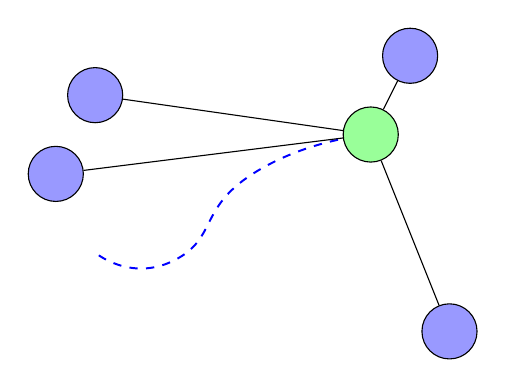
\begin{tikzpicture}[auto, node distance=1cm,>=latex']
\draw [cyan, line width=0.25mm, dashed, color=blue] plot [smooth, tension=1] coordinates { (2.5,1.5) (1,1) (0,-0.1) (-1, 0)};

\node[circle,draw, minimum size=0.7cm, fill=green!40!white] (A) at  (2.5,1.5)  {};

\node[circle,draw, minimum size=0.7cm, fill=blue!40!white] (B) at  (3.5,-1) {};
\node[circle,draw, minimum size=0.7cm, fill=blue!40!white] (C) at  (-1,2) {};
\node[circle,draw, minimum size=0.7cm, fill=blue!40!white] (D) at  (3,2.5) {};
\node[circle,draw, minimum size=0.7cm, fill=blue!40!white] (E) at  (-1.5,1) {};

\draw (A) -- (B);
\draw (A) -- (C);
\draw (A) -- (D);
\draw (A) -- (E);

\end{tikzpicture}
\end{center}
\end{frame}

\begin{frame}[t]{Geometric Dilution of Precision}

\small
\begin{columns}
\column{0.5\textwidth}

\begin{itemize}
  \item Conveniently, as we have set up the problem here, Geometric Dilution of Precision (GDOP) is a convenient proxy for "information" we are interested.
  \item GDOP is a measure of the sensitivity of measurement error on the output position, as a function of the geometries of the agents. A lower GDOP value is prefered.
  \item In our 2D example, GDOP is calculated as follows:
  \[ A = \begin{bmatrix} \frac{x_1 - x}{R_1}& \frac{y_1 - x}{R_1} & -1\\ &\vdots \\  \frac{x_n - x}{R_n} & \frac{y_n - x}{R_n} & -1\\ \end{bmatrix} \]
  \[ \text{GDOP}  = tr\{ (A^T A)^{-1} \}\]
  \item This metric is commonly used in sattelite positioning, which also relies on ranging.
\end{itemize}

\column{0.5\textwidth}

\begin{figure}
\includegraphics[width=0.7\textwidth,right]{img/bad_gdop.png}
\caption{Example of poor spatial diversity, high dilution of precision.}
\end{figure}
\begin{figure}
\includegraphics[width=0.9\textwidth,right]{img/good_gdop.png}
\caption{Example of good spatial diversity, low dilution of precision.}
\end{figure}
\end{columns}

\end{frame}

\begin{frame}{Problem Formulation}

\begin{columns}
\column{0.5\textwidth}

\begin{itemize}
  \item The goal is to minimize the objective function
  \[J = \phi(x(t), u(t), t),\]
  subject to dynamic constraints
  \[\dot{x} = Ax + u\]
  and path constraints
  \[c(x(t), u(t), t) \leq 0\]
  \item The state, $x$, contains the states of all the agents and is jointly optimized.
  \[ x = \left[x_1, y_1, \dot{x}_1, \dot{y}_1, ~..., x_n, y_n, \dot{x}_n, \dot{y}_n \right]^T \]
  % \item 
\end{itemize}

\column{0.5\textwidth}

\begin{figure}
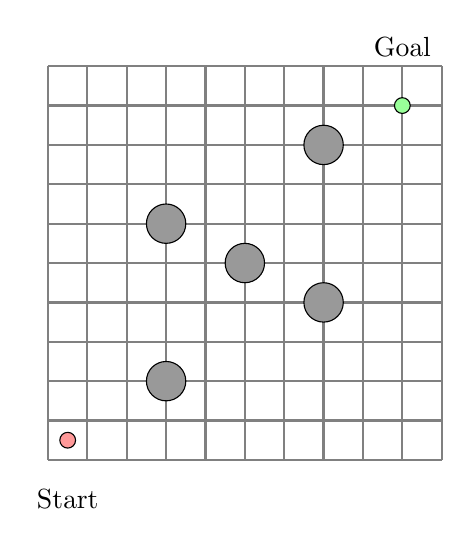
\begin{tikzpicture}[auto, node distance=1cm,>=latex']
\draw (0, 0) -- (5, 0) -- (5, 5) -- (0,5) -- (0, 0);
\draw[step=0.5,gray,thick] (0,0) grid (5,5);

% obstacles
\draw[black,fill=black!40!white] (1.5, 1) circle (0.25);
\draw[black,fill=black!40!white] (3.5, 2) circle (0.25);
\draw[black,fill=black!40!white] (1.5, 3) circle (0.25);
\draw[black,fill=black!40!white] (3.5, 4) circle (0.25);
\draw[black,fill=black!40!white] (2.5, 2.5) circle (0.25);

\draw[black,fill=red!40!white] (0.25, 0.25) circle (0.1);
\node[align=center] at (0.25, -0.5) {Start};

\draw[black,fill=green!40!white] (4.5, 4.5) circle (0.1);
\node[align=left] at (4.5, 5.25) {Goal};

\end{tikzpicture}
\caption{\tiny Example of the map. The red and green points denote the start and goal, respectively. The gray points indicate obstacles that the final paths may not intersect.}
\end{figure}

\end{columns}

\end{frame}

\begin{frame}[t]{State Dynamics and Constraints}

\begin{itemize}
  \item Agents have full control authority in each dimension of their state.
  \[ \begin{bmatrix} \dot{x}_1 \\ \dot{y}_1 \\ \ddot{x}_1 \\ \ddot{y}_1 \\ \vdots \\ \dot{x}_n \\ \dot{y}_n \\ \ddot{x}_n \\ \ddot{y}_n \end{bmatrix}= \begin{bmatrix} 0 & 0 & 1 & 0 \\ 0 & 0 & 0 & 1 & \dots \\ 0 & 0 & 0 & 0 \\ 0 & 0 & 0 & 0 \\ \vdots & & & & \ddots \\ & & & & & 0 & 0 & 1 & 0 \\ & & & & & 0 & 0 & 0 & 1 \\& & & & &  0 & 0 & 0 & 0 \\& & & & &  0 & 0 & 0 & 0 \end{bmatrix} \begin{bmatrix} x_1 \\ y_1 \\ \dot{x}_1 \\ \dot{y}_1 \\ \vdots \\ x_n \\ y_n \\ \dot{x}_n \\ \dot{y}_n \end{bmatrix} + \begin{bmatrix} 0 \\ 0 \\ u_{x_1} \\ u_{y_1} \\ \vdots \\ 0 \\ 0 \\ u_{x_n} \\ u_{y_n}\end{bmatrix}\]
  \item The control is constrained.
  \[ u_{\text{min}} \leq u \leq u_{\text{max}} \]
  \item The secondary agents must be within the communication range of the primary agent.
  \[ d(t) \leq r_{\text{max}} \]
  \item The final paths may not intersect with any obstacles, $O$.
  \[ x(t) \cap O \leq 0\]
\end{itemize}

\end{frame}

% \begin{frame}{GPOPS-II Implementation}
% \begin{itemize}
%   \item Objectives to minimize:
%   \begin{itemize}
%     \item Total time
%     \item Total control effort
%     \item Primary agent's position dilution of precision
%   \end{itemize}
%   \item Bounds
%   \begin{itemize}

%   \end{itemize}
% \end{itemize}
% \end{frame}

% -----------------------------------------------------------------------------

\begin{frame}{Results}
\begin{figure}
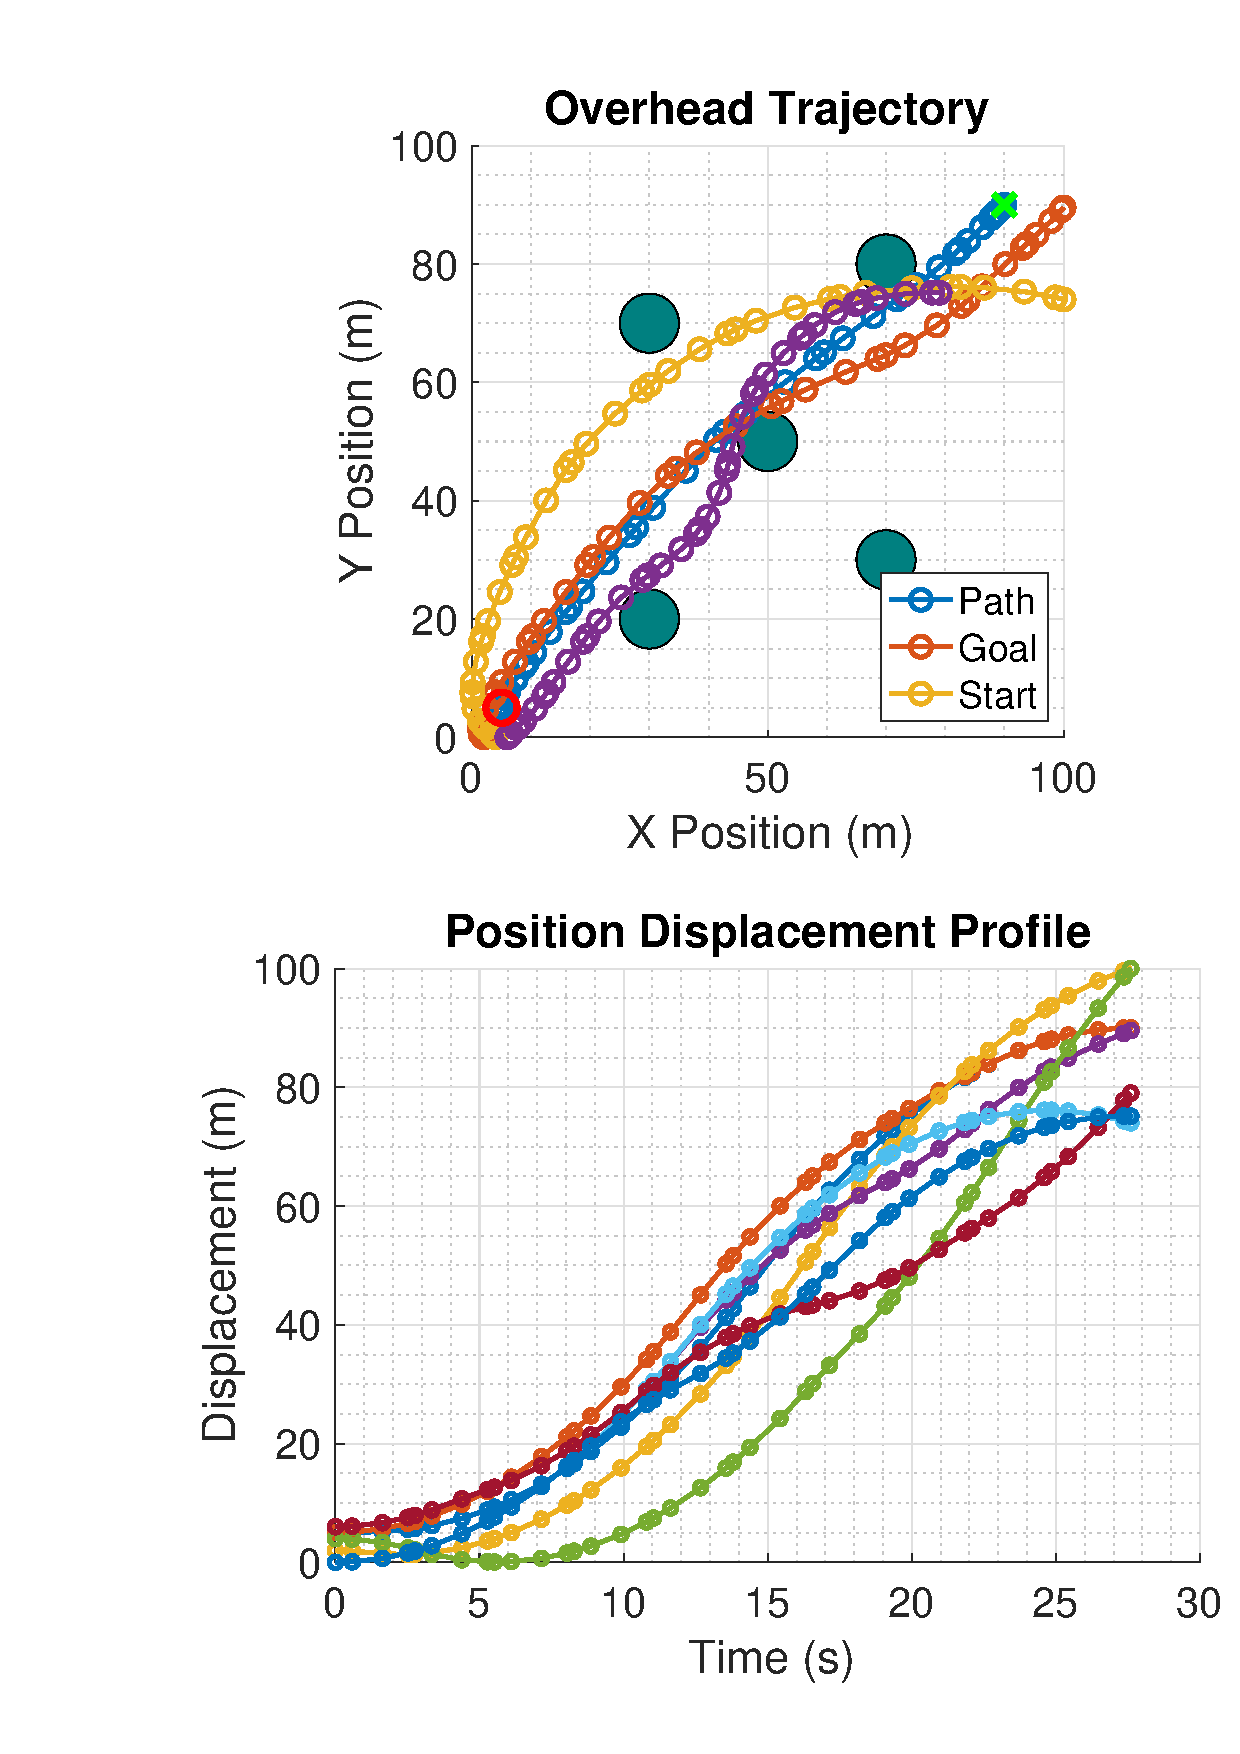
\includegraphics[width=\textwidth]{img/results.png}
\caption{GPOPS-II results for optimal paths.}
\end{figure}
\end{frame}

\begin{frame}{Conclusion}
\begin{itemize}
  \item This projects uses GPOPS-II to optimize the paths of a multi-agent system, in a manner that attempts to maximize information.
  \item We can jointly solve for the optimal paths under the provided constraints. And we find that GDOP is a useful 'information' metric, for the solver.
  \item Future Work:
  \begin{itemize}
    \item How could this be implemented in a decentralized manner?
    \item Are there methods to implemt this type of control in real-time, operating in dynamic environments?
    \item How could we extend the 'information' metric more generally to other types of nonlinear sensors? (i.e. bearing)
    \item Investigate complex agent dynamics.
  \end{itemize}
\end{itemize}
\begin{itemize}

\end{itemize}
\end{frame}

\begin{frame}{References}
\begin{itemize} \small
  \item \url{https://en.wikipedia.org/wiki/Dilution_of_precision_(navigation)}
  \item F. Meyer, H. Wymeersch, M. Fröhle and F. Hlawatsch, "Distributed Estimation With Information-Seeking Control in Agent Networks," in IEEE Journal on Selected Areas in Communications, vol. 33, no. 11, pp. 2439-2456, Nov. 2015, doi: 10.1109/JSAC.2015.2430519.
  \item J. Spletzer, A. K. Das, R. Fierro, C. J. Taylor, V. Kumar and J. P. Ostrowski, "Cooperative localization and control for multi-robot manipulation," Proceedings 2001 IEEE/RSJ International Conference on Intelligent Robots and Systems. Expanding the Societal Role of Robotics in the the Next Millennium (Cat. No.01CH37180), Maui, HI, USA, 2001, pp. 631-636 vol.2, doi: 10.1109/IROS.2001.976240.
\end{itemize}
\end{frame}

\end{document}
